\documentclass[a4paper, titlepage]{article}
\usepackage[utf8]{inputenc}
\usepackage{hyperref}
\usepackage{xcolor}
\hypersetup{
	colorlinks,
	linkcolor={red!50!black},
	urlcolor={blue!80!black}
}
\usepackage{graphicx}
\graphicspath{ {images/} }
\title{Tom's Git Guide}
\author{Tom Schwarz, Ben Schwarz}
\date{Janurary 2019\\v1.A} %letters for pre-releases, .0 for main release, .1+ for post-updates

\begin{document}
\maketitle

\tableofcontents

\renewcommand{\abstractname}{Introduction} %changes the abstract to be called an introduction.
\begin{abstract}
This guide was written to explain how to use git (and GitHub) quickly and easily. While it definitely is not a particularly good guide, I couldn't find one online that explained, practically, how to use git with the right context and simply enough. So I wrote this. For an explanation of how Git works (which you \emph{must} know before you read this (knowing ``git commit'', ``git pull'' and ``git push'' or their equivalent GUI buttons dosen't count)) see \href{https://blog.red-badger.com/2016/11/29/gitgithub-in-plain-english}{Git \& Github in plain english} (seriously - do read it).
\end{abstract}

\section{Solving merge conflicts}

\section{Branching \& Pull Request Workflow}
This explains a simple workflow, but in extreme detail. A quick outline of this workflow:
\begin{enumerate}
	\item Create a branch and work on your new changes there
	\item Create a pull request to incorporate changes into master
	\item Review \& approve the pull request, making changes as necessary
	\item Delete the branch
\end{enumerate}
\subsection{Creating a branch}
\begin{enumerate}
	\item Make sure your git repo is up to date with origin (ie Github) - either by running ``git pull'' or in the GUI clicking the ``Fetch origin'' button
	\item Create the branch by running ``git checkout -b your-branch-name'' or in the GUI going ``Branch \textgreater New Branch'' (also available from the ``current branch'' button next to fetch origin).
	\item Choose a suitable branch name, compliant with relevant conventions/guidelines - it should be short and descriptive. You should create a new branch for every self-contained feature - do NOT create large monolithic branches for miscellaneous updates; even if it means having a branch with just one commit.
	\item Add this branch to origin either by running ``git push --set-upstream origin your-branch-name'' (the extra option connects your new branch to a new reflected branch in origin) or hitting the ``Publish branch'' button in the GUI.
	\begin{figure}[h]
		\centering
		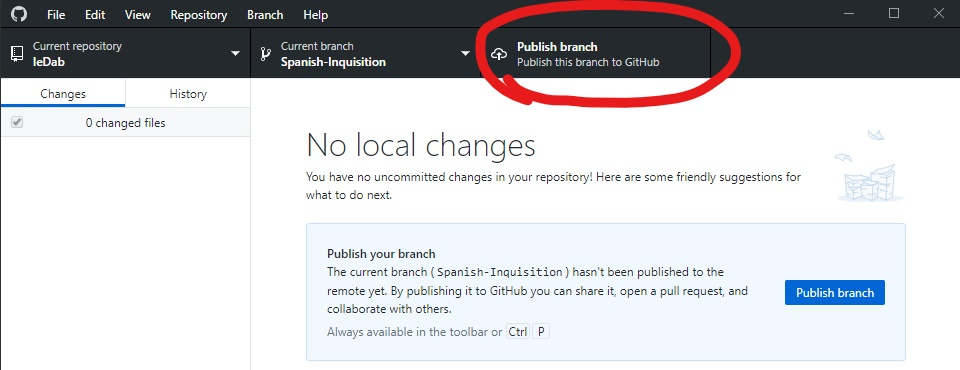
\includegraphics[width=\textwidth]{1publish-branch}
		\caption{The publish branch button in the GUI}
	\end{figure}
	\item Now you can start working on your feature, updating code, making commits and pushing them up to Github as normal!
\end{enumerate}

\subsection{Creating the pull request}
temp

\subsection{Reviewing the pull request}
temp

\subsubsection{Making changes}
temp

\subsubsection{Approving the pull request}
temp

\subsection{cleanup}
temp

\end{document}